\documentclass[aspectratio=169,11pt]{beamer}
\usetheme{Madrid}
\usecolortheme{seahorse}
\usepackage[T1]{fontenc}
\usepackage[utf8]{inputenc}
\usepackage{booktabs}
\usepackage{tikz}
\usetikzlibrary{arrows.meta,positioning,shapes.geometric}
\usepackage{multicol}

\setbeamertemplate{navigation symbols}{}
\setbeamertemplate{footline}[frame number]

\title{Labyrinth Breach}
\subtitle{Reinforcement Learning-based Multi-Agent Pursuit-Evasion\\in Dynamic Maze Environments}
\author{Muhammad Sikander Raheem \quad Usman Irshad Bhatti \quad Ahmed Jawed}
\institute{MS AI, LUMS | AI641 -- AI for Robotics}
\date{May 2025}

\begin{document}

% ============ SLIDE 1: TITLE ============
\begin{frame}
\titlepage
\vspace{-10pt}
\begin{center}
{\small Unity ML-Agents \quad|\quad PPO \quad|\quad MARL}
\end{center}
\end{frame}

% ============ SLIDE 2: PROJECT OVERVIEW ============
\begin{frame}{Project Overview}
\begin{columns}[T]
\column{0.5\textwidth}
\textbf{What is Labyrinth Breach?}
\begin{itemize}
\item \textbf{Environment:} Unity ML-Agents maze simulator
\item \textbf{Setup:} 3 Sentinels vs 2 Runners (3v2 asymmetric)
\item \textbf{Goal (Sentinels):} Capture both Runners before timeout
\item \textbf{Goal (Runners):} Reach an exit zone or survive 120s
\item \textbf{Mazes:} Procedurally generated with dynamic wall shifts
\end{itemize}

\column{0.5\textwidth}
\textbf{Key Technical Challenges}
\begin{itemize}
\item \textbf{Partial Observability} -- Raycasts + last-known-position memory; no global state
\item \textbf{Multi-Agent Coordination} -- 3 agents must cooperate to trap 2 evaders
\item \textbf{Dynamic Environment} -- Walls shift mid-episode, forcing real-time adaptation
\item \textbf{Asymmetric Teams} -- Different team sizes, roles, reward structures
\item \textbf{Generalization} -- Must work on unseen maze layouts
\end{itemize}
\end{columns}
\end{frame}

% ============ SLIDE 3: LIT REVIEW OVERVIEW ============
\begin{frame}{Literature Review -- Foundations \& Related Work}
\begin{center}
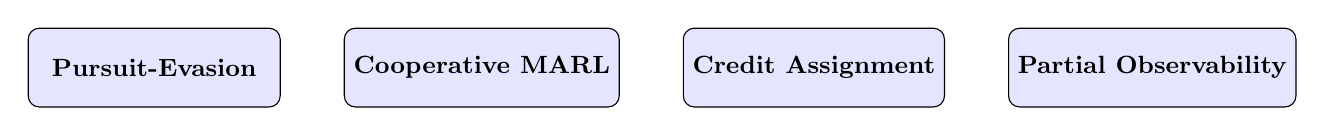
\begin{tikzpicture}[
  theme/.style={draw, rounded corners, fill=blue!10, minimum width=3.2cm, minimum height=1cm, align=center, font=\small\bfseries},
  node distance=0.8cm
]
\node[theme] (pe) {Pursuit-Evasion};
\node[theme, right=of pe] (coop) {Cooperative MARL};
\node[theme, right=of coop] (credit) {Credit Assignment};
\node[theme, right=of credit] (po) {Partial Observability};
\end{tikzpicture}
\end{center}
\vspace{6pt}
\begin{columns}[T]
\column{0.25\textwidth}
{\small Route blocking, pincer, spatial entrapment, escape timing}
\column{0.25\textwidth}
{\small Non-stationarity, CTDE, parameter sharing, PPO baselines}
\column{0.25\textwidth}
{\small Shared reward too coarse, counterfactual baselines, reward shaping}
\column{0.25\textwidth}
{\small LOS constraints, memory, uncertainty changes optimal strategies}
\end{columns}
\end{frame}

% ============ SLIDE 4: THEME 1 ============
\begin{frame}{Theme 1 -- Pursuit-Evasion as a Multi-Agent Problem}
\begin{columns}[T]
\column{0.55\textwidth}
\textbf{Core Concept}\\
Classical robotics and MARL problem: one side captures, the other evades. RL is a natural fit because desired behavior is hard to hand-code under adversarial interaction, obstacles, and partial information.

\vspace{6pt}
\textbf{Richer Behaviors Required}
\begin{columns}[T]
\column{0.5\textwidth}
\textit{Sentinel:}
\begin{itemize}
\item Trapping and pincer
\item Corridor denial
\item Exit blocking
\item Route cutting
\end{itemize}
\column{0.5\textwidth}
\textit{Runner:}
\begin{itemize}
\item Distance management
\item Path selection
\item Survival timing
\item Exploit topology
\end{itemize}
\end{columns}

\column{0.45\textwidth}
\textbf{Key References}

\textbf{Verma et al. (2019)} -- Multi-agent pursuer-evader learning; emergent route-blocking from simple rewards.

\textbf{Yan et al. (2019)} -- Pursuit-evasion with uncertain pursuer speeds; coordination under real-world constraints.

\textbf{Liu et al. (2024)} -- Multi-UAV pursuit-evasion via PSO-M3DDPG; large-scale aerial coordination.

\textbf{Haeri et al. (2022)} -- Emergent behaviors in multi-agent target acquisition; rich behavior from simple reward signals.
\end{columns}
\end{frame}

% ============ SLIDE 5: THEME 2 ============
\begin{frame}{Theme 2 -- Cooperative \& Mixed Multi-Agent RL}
\textbf{Core Challenge: Non-Stationarity} -- All agents update simultaneously; each agent's environment is non-stationary, making standard RL convergence guarantees inapplicable.

\vspace{6pt}
\begin{columns}[T]
\column{0.33\textwidth}
\textbf{MADDPG} {\small(Lowe et al., 2017)}\\[3pt]
Centralized Training, Decentralized Execution (CTDE): actor uses local obs, critic accesses global state.\\[4pt]
{\small\textit{Our use:} CTDE principle; we use PPO's parameter sharing as a simpler alternative.}

\column{0.33\textwidth}
\textbf{MAPPO} {\small(Yu et al., 2022)}\\[3pt]
Well-tuned PPO surprisingly outperforms complex algorithms in cooperative MARL. Lower complexity, better reproducibility.\\[4pt]
{\small\textit{Our use:} Primary training method; Unity ML-Agents provides native PPO support.}

\column{0.33\textwidth}
\textbf{Parameter Sharing}\\[3pt]
Agents within a team share a single policy network. Reduces sample complexity and enforces role symmetry.\\[4pt]
{\small\textit{Our use:} 3 Sentinels share one policy; 2 Runners share another -- distinct from each other.}
\end{columns}
\end{frame}

% ============ SLIDE 6: THEME 3 ============
\begin{frame}{Theme 3 -- Credit Assignment in Cooperative MARL}
\begin{columns}[T]
\column{0.45\textwidth}
\textbf{The Credit Assignment Problem}\\
When multiple agents cooperate under team-level objectives, one may contribute by blocking a route while another captures. Plain shared reward is too coarse -- agents cannot distinguish meaningful contributions from free-riding.

\vspace{6pt}
\textbf{Our Approach}\\
Tactical reward shaping with per-agent bonuses for coordination events: pincer formations, corridor control, exit denial, and dead-end forcing.

\column{0.55\textwidth}
\textbf{Landmark Solutions}

\begin{tabular}{@{}p{4.5cm}p{2cm}@{}}
\toprule
\textbf{Method} & \textbf{Type} \\
\midrule
QMIX (Rashid 2018) -- monotonic value factorisation & Value decomp. \\
COMA (Foerster 2018) -- counterfactual baseline & Gradient-based \\
Implicit Credit (Wang 2020) -- attention over teammates & Attention \\
Polarization PG (Chen 2023) -- explicit credit via gradient polarity & Explicit \\
\bottomrule
\end{tabular}
\end{columns}
\end{frame}

% ============ SLIDE 7: THEME 4 ============
\begin{frame}{Theme 4 -- Partial Observability in Pursuit-Evasion}
\textbf{Why it matters:} With full global state, pursuit-evasion becomes a trivial tracking problem. Partial observability forces agents to plan under uncertainty, maintain beliefs, and use memory.

\vspace{6pt}
\begin{columns}[T]
\column{0.5\textwidth}
\textbf{ViPER} {\small(Wang, Sartoretti \& How, 2025)}\\
Visibility-based PE via RL. Agents observe only within a line-of-sight cone.\\[3pt]
\textit{Key insight:} LOS constraints fundamentally change optimal strategies.\\[3pt]
{\small\textit{vs. Ours:} We add team coordination (3v2) and dynamic topology.}

\column{0.5\textwidth}
\textbf{Gonultas \& Isler (2024)}\\
PE with dynamic sensor and actuation constraints. Limited range, noise, uncertain speeds.\\[3pt]
\textit{Key insight:} Uncertainty about opponent dynamics is as important as sensing range.\\[3pt]
{\small\textit{vs. Ours:} Our memory-augmented obs addresses uncertainty at a system level.}
\end{columns}

\vspace{6pt}
\begin{center}
{\small\textbf{Our pipeline:} vector state + 360\textdegree{} raycasts (14 Sentinel / 16 Runner rays) + last-known-position memory $\rightarrow$ 117 / 129 float observation vectors}
\end{center}
\end{frame}

% ============ SLIDE 8: SYNTHESIS ============
\begin{frame}{Synthesis -- How the Literature Shapes Our Design}
\begin{center}
\begin{tabular}{@{}p{2.5cm}p{5cm}p{4.5cm}@{}}
\toprule
\textbf{Theme} & \textbf{Key Insight} & \textbf{Design Decision} \\
\midrule
Pursuit-Evasion & Rich behaviors emerge in topologically complex environments & Procedural maze + exit zones + dynamic walls \\[4pt]
Cooperative MARL & PPO with parameter sharing is a competitive baseline & Shared policy per team, PPO via Unity ML-Agents \\[4pt]
CTDE & Centralized critic resolves non-stationarity & MA-POCA supported; PPO used in reported experiments \\[4pt]
Credit Assignment & Shared reward too coarse for indirect contributions & Tactical shaping: pincer, corridor, exit denial \\[4pt]
Partial Observability & LOS + memory changes strategy fundamentally & Raycasts + last-known-position; no global state \\
\bottomrule
\end{tabular}
\end{center}
\end{frame}

% ============ SLIDE 9: POSG ============
\begin{frame}{Problem Formulation}
\textbf{Partially Observable Stochastic Game (POSG)}\\[3pt]
$\langle N, \mathcal{S}, \{A_i\}, \{O_i\}, T, \{R_i\}, \gamma \rangle$ where $N{=}5$, $\gamma{=}0.99$

\vspace{6pt}
The joint state covers positions, velocities, and wall configuration. The transition function is governed by Unity's physics engine.

\vspace{6pt}
\textbf{Asymmetric, team-versus-team interaction:}
\begin{itemize}
\item \textbf{Sentinels win} when both Runners are captured before timeout
\item \textbf{Runners win} when one reaches an exit, or by surviving 120s (5,000 steps)
\end{itemize}

\vspace{6pt}
Zero-sum between teams but cooperative within teams -- this is the core reason it is a multi-agent learning problem, not just two single-agent problems.
\end{frame}

% ============ SLIDE 10: ENVIRONMENT ============
\begin{frame}{Environment Design}
The environment is built in Unity ML-Agents and structured as \textbf{four scenes} of increasing difficulty:

\vspace{4pt}
\begin{center}
\begin{tabular}{@{}lcl@{}}
\toprule
\textbf{Scene} & \textbf{Walls} & \textbf{Purpose} \\
\midrule
01\_Baseline\_OpenArena\_3v2 & None & Basic pursuit mechanics \\
02\_StaticMaze\_3v2 & Fixed & Navigation and route-cutting \\
03\_DynamicMaze\_3v2 & Shift every 8--20s & Adaptation to topology changes \\
04\_Eval\_UnseenMaze\_3v2 & Novel layout & Generalization testing \\
\bottomrule
\end{tabular}
\end{center}

\vspace{6pt}
\textbf{Dynamic wall mechanics:} Each wall is a vertical pillar that can rise or sink. The controller picks two random pillars and toggles them, but only after a safety check that prevents shifting walls within 1.75m of any agent and prevents sealing exits.

\vspace{4pt}
Topology mutates during play, but never produces unfair states or unreachable goals.
\end{frame}

% ============ SLIDE 11: OBSERVATIONS ============
\begin{frame}{Agent Observations and Actions}
\begin{columns}[T]
\column{0.5\textwidth}
\textbf{Observation Vector}
\begin{tabular}{@{}lcc@{}}
\toprule
\textbf{Component} & \textbf{Sent.} & \textbf{Run.} \\
\midrule
Self state (pos, vel, heading, alive) & 10 & 10 \\
Env context (time, exit, wall) & 7 & 7 \\
Last-known-position memory & 6 & 6 \\
Rays ($N \times 6$ floats) & 84 & 96 \\
Opponent summary ($2 \times 5$) & 10 & 10 \\
\midrule
\textbf{Total} & \textbf{117} & \textbf{129} \\
\bottomrule
\end{tabular}

\vspace{6pt}
Each ray = 6 floats: normalized distance + one-hot (wall, exit, teammate, opponent, other).

\column{0.5\textwidth}
\textbf{Action Space}\\
2 continuous values, each clamped to $[-1, 1]$, interpreted as 2D world-frame velocity in the XZ plane.

\vspace{6pt}
\textbf{Design Decisions}
\begin{itemize}
\item \textbf{No camera/pixels} -- vector observations train 10x faster and are fully interpretable
\item \textbf{No global state} -- agents never see the full maze, making this a true POSG
\item \textbf{Memory} -- stores last-known XYZ when target leaves LOS, decays over time
\item \textbf{More Runner rays} (16 vs 14) -- prey needs wider threat detection
\end{itemize}
\end{columns}
\end{frame}

% ============ SLIDE 12: REWARDS ============
\begin{frame}{Reward Design}
\textbf{Three reward layers:}

\vspace{4pt}
\begin{columns}[T]
\column{0.33\textwidth}
\textbf{1. Terminal Layer}\\
{\small Shared team reward of $\pm$1.0. Every Sentinel gets $+1.0$ if both Runners captured; every Runner gets $+1.0$ if one escapes or timeout.}

\column{0.33\textwidth}
\textbf{2. Shaping Layer}\\
{\small Per-agent: chase/evade progress ($\sim$1e-3/step), plus penalties for wall-loops, orbit-stalls, threat approaches. Mitigates lazy-agent failure mode.}

\column{0.33\textwidth}
\textbf{3. Tactical Layer}\\
{\small Coalition-scoped: pincer rewards the 2 Sentinels involved; corridor control rewards blockers; exit denial rewards the guarding Sentinel. Cluster penalty discourages bunching.}
\end{columns}

\vspace{6pt}
\begin{center}
\textbf{Pipeline:} YAML config $\rightarrow$ RewardConfig $\rightarrow$ Role-specific Policy $\rightarrow$ RewardEngine $\rightarrow$ agent.AddReward() $\rightarrow$ StepLogger (CSV audit)
\end{center}
\end{frame}

% ============ SLIDE 13: TRAINING ============
\begin{frame}{Training Algorithm \& Architecture}
\begin{columns}[T]
\column{0.5\textwidth}
\textbf{PPO with Parameter Sharing}
\begin{itemize}
\item 2 policies total (not 5): one Sentinel brain, one Runner brain
\item All 3 Sentinels share same weights; both Runners share another
\item Coordination emerges from differing observations of the same policy
\item 3$\times$ sample throughput on Sentinel side per environment step
\end{itemize}

\vspace{4pt}
\textbf{Network Architecture}\\
Shared-backbone actor-critic MLP:
\begin{itemize}
\item Input $\rightarrow$ 256 units (Swish) $\rightarrow$ 256 units (Swish)
\item Actor head $\rightarrow$ 2 floats (Gaussian mean + learned std)
\item Critic head $\rightarrow$ 1 float (state value $V(s)$)
\item $\sim$100K parameters per brain
\end{itemize}

\column{0.5\textwidth}
\textbf{PPO Hyperparameters}
\begin{tabular}{@{}lr@{}}
\toprule
Parameter & Value \\
\midrule
Learning rate & $3 \times 10^{-4}$ (linear decay) \\
Batch size & 1024 \\
Buffer size & 10240 \\
Hidden layers & 2 $\times$ 256 \\
Epochs & 3 \\
$\gamma$ & 0.99 \\
$\lambda$ (GAE) & 0.95 \\
$\epsilon$ (clip) & 0.2 \\
$\beta$ (entropy) & 0.005 \\
Time horizon & 64 \\
Max steps & 500K \\
Optimizer & Adam \\
\bottomrule
\end{tabular}

\vspace{2pt}
{\small Follows MAPPO recipe (Yu et al., 2022)}
\end{columns}
\end{frame}

% ============ SLIDE 14: CURRICULUM ============
\begin{frame}{Curriculum}
Training is staged. Each stage has both a \textbf{minimum-episode threshold} and a \textbf{Sentinel-win-rate gate}. Agents advance only when both are satisfied -- the curriculum is adaptive, not on a fixed schedule.

\vspace{6pt}
\begin{center}
\begin{tabular}{@{}lcccc@{}}
\toprule
\textbf{Stage} & \textbf{Min Episodes} & \textbf{Walls} & \textbf{Win Rate Gate} & \textbf{Purpose} \\
\midrule
1. Static, fixed spawns & 1,200 & None & 0.62 & Basic pursuit mechanics \\
2. Static, random spawns & 2,200 & None & 0.55 & Prevent route memorization \\
3. Dynamic, 20s shifts & 3,200 & 20s & 0.50 & Slow topology adaptation \\
4. Dynamic, 8s shifts & 3,000 & 8s & 0.45 & Fast real-time replanning \\
\bottomrule
\end{tabular}
\end{center}

\vspace{6pt}
\textbf{Motivation} (Zhang et al., 2023): Coordination behaviors are hard to discover from sparse reward in the full-difficulty environment but easier to bootstrap in simpler ones, then transfer.
\end{frame}

% ============ SLIDE 15: ARCHITECTURE ============
\begin{frame}{System Architecture}
\begin{center}
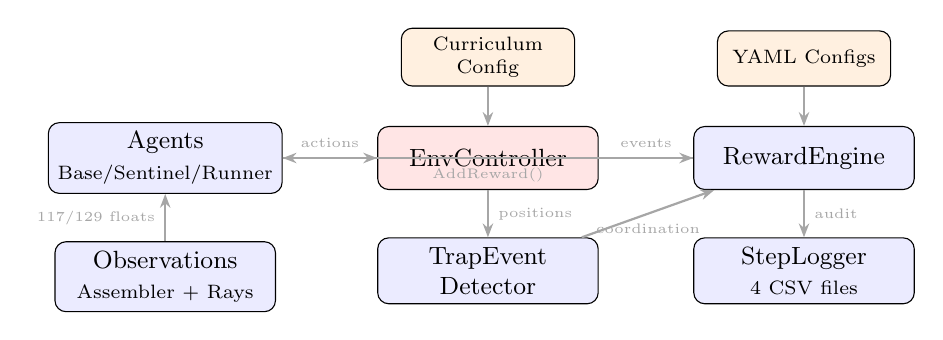
\begin{tikzpicture}[
  box/.style={draw, rounded corners, fill=blue!8, minimum width=2.8cm, minimum height=0.8cm, align=center, font=\small},
  configbox/.style={draw, rounded corners, fill=orange!12, minimum width=2.2cm, minimum height=0.7cm, align=center, font=\scriptsize},
  arrow/.style={-{Stealth[length=5pt]}, thick, color=gray!70},
  node distance=0.6cm and 0.8cm
]
  \node[box, fill=red!10] (ctrl) {EnvController};
  \node[box, left=1.2cm of ctrl] (agents) {Agents\\{\scriptsize Base/Sentinel/Runner}};
  \node[box, right=1.2cm of ctrl] (reward) {RewardEngine};
  \node[box, below=of agents] (obs) {Observations\\{\scriptsize Assembler + Rays}};
  \node[box, below=of ctrl] (trap) {TrapEvent\\Detector};
  \node[box, below=of reward] (log) {StepLogger\\{\scriptsize 4 CSV files}};
  \node[configbox, above=0.5cm of reward] (yaml) {YAML Configs};
  \node[configbox, above=0.5cm of ctrl] (curriculum) {Curriculum\\Config};

  \draw[arrow] (agents) -- (ctrl) node[midway,above,font=\tiny] {actions};
  \draw[arrow] (ctrl) -- (reward) node[midway,above,font=\tiny] {events};
  \draw[arrow] (reward) -- (agents.east|-reward) node[midway,below,font=\tiny] {AddReward()};
  \draw[arrow] (obs) -- (agents) node[midway,left,font=\tiny] {117/129 floats};
  \draw[arrow] (ctrl) -- (trap) node[midway,right,font=\tiny] {positions};
  \draw[arrow] (trap) -- (reward) node[midway,below,font=\tiny] {coordination};
  \draw[arrow] (reward) -- (log) node[midway,right,font=\tiny] {audit};
  \draw[arrow] (yaml) -- (reward);
  \draw[arrow] (curriculum) -- (ctrl);
\end{tikzpicture}
\end{center}
\vspace{-4pt}
{\small\textbf{Key design:} Everything is config-driven. Change reward weights, curriculum thresholds, or observation setup without touching C\# code.}
\end{frame}

% ============ SLIDE 16: AGENT HIERARCHY ============
\begin{frame}{Agent Hierarchy}
\begin{columns}[T]
\column{0.5\textwidth}
\textbf{Inheritance Chain}
\begin{itemize}
\item \texttt{Unity.MLAgents.Agent}
  \begin{itemize}
  \item \texttt{BaseAgent} -- movement, observation, ML-Agents hooks
    \begin{itemize}
    \item \texttt{SentinelAgent} -- capture radius, target tracking
    \item \texttt{RunnerAgent} -- escape logic, captured state
    \end{itemize}
  \end{itemize}
\end{itemize}

\vspace{6pt}
\textbf{Parameter Sharing}
\begin{itemize}
\item All 3 Sentinels $\rightarrow$ one PPO brain
\item Both Runners $\rightarrow$ one PPO brain
\item Same weights, different observations
\item What one agent learns, all agents know
\end{itemize}

\column{0.5\textwidth}
\textbf{ML-Agents Lifecycle (every step)}
\begin{enumerate}
\item \textbf{Observe} -- build the 117/129 float vector from sensors, rays, and memory
\item \textbf{Decide} -- neural network maps observation $\rightarrow$ 2 continuous actions
\item \textbf{Act} -- apply movement to the agent's rigidbody
\item \textbf{Reward} -- RewardEngine computes and assigns reward
\item \textbf{Log} -- StepLogger records the event to CSV
\end{enumerate}

\vspace{6pt}
\textbf{Episode boundaries}
\begin{itemize}
\item Start: agents reset position and memory
\item End: both captured, exit reached, or 120s timeout
\end{itemize}
\end{columns}
\end{frame}

% ============ SLIDE 17: LOGGING ============
\begin{frame}{Logging \& Evaluation}
\begin{columns}[T]
\column{0.5\textwidth}
\textbf{4 CSV Output Files}
\begin{enumerate}
\item \texttt{episode\_log.csv} -- outcome, duration, captured count
\item \texttt{agent\_step\_log.csv} -- per-agent XYZ every step
\item \texttt{reward\_audit.csv} -- every reward event with type and value
\item \texttt{replay\_events.csv} -- captures, escapes, tactical events
\end{enumerate}

\vspace{6pt}
\textbf{Evaluation Protocol}
\begin{itemize}
\item 3 seeds: 42, 101, 202
\item Seen layouts (training mazes)
\item Unseen layouts (novel procedural mazes)
\item Metrics averaged across seeds
\end{itemize}

\column{0.5\textwidth}
\textbf{Results}
\begin{tabular}{@{}lcc@{}}
\toprule
Metric & Seen & Unseen \\
\midrule
Sentinel WR & 62.0\% & 60.3\% \\
1st capture & 17.2s & 9.7s \\
2nd capture & 37.8s & 24.5s \\
Escape frac & 26.0\% & 26.8\% \\
Timeout surv & 12.0\% & 12.9\% \\
\bottomrule
\end{tabular}

\vspace{6pt}
\textbf{Key insight:}\\
Win rates transfer (1.7pt drop).\\
Capture timing shifts (7.5s faster).\\
\textit{Policies are topology-sensitive but not layout-memorized.}
\end{columns}
\end{frame}

% ============ SLIDE 18: SUMMARY ============
\begin{frame}{Summary}
\begin{columns}[T]
\column{0.5\textwidth}
\textbf{What makes this more than a toy project:}
\begin{itemize}
\item Modular architecture (agents, rewards, sensors, logging are all separate)
\item Config-driven (YAML for everything: rewards, curriculum, PPO, evaluation)
\item Full audit trail (4 CSV logs track every reward, every step, every event)
\item Reproducible (3 seeds, seen/unseen split, public repo)
\item Dynamic environment (walls shift during episodes)
\end{itemize}

\column{0.5\textwidth}
\textbf{Honest limitations:}
\begin{itemize}
\item No MA-POCA comparison yet (credit assignment)
\item No ablation study (memory on/off, shaping on/off)
\item Coordination is observed qualitatively but not quantified with dedicated metrics
\item BufferSensor path exists but is untested
\end{itemize}

\vspace{6pt}
\textbf{Repo:} \texttt{github.com/ahmedjawedaj/labyrinth-breach-marl}
\end{columns}
\end{frame}

\end{document}
